\appendix

\section*{Anhang}
\addcontentsline{toc}{section}{Anhang}

% um numerierung im anhang trotzdem zu erhalten
\renewcommand{\thesubsection}{\Alph{subsection}}
% notation von abbildungen wird geänder: 1 > A.1 
\renewcommand{\thefigure}{\thesubsection.\arabic{figure}}
%an dieser stelle würde ich gern die notation von listings im anhang anpassen, bisher aber leider erfolglos

% berichtigen des counters für abbildungen
\setcounter{figure}{0}

\subsection{Nachbereitung}

Als allererstes, hier noch die letzte Referenz zum folgenden Listing im Anhang: \ref{lst:helloworld}  
Die hier benutzte Arbeit entstand im Rahmen des Moduls \textit{Wissenschaftliches Arbeiten} aus dem 
4. Semester. Da keine Bilder oder Grafiken vorgesehen waren, habe ich ein paar eher weniger relevante 
eingefügt. Trotzdem hoffe ich, dass der Leseflow der Arbeit einigermaßen angenehm ist. Alle für diese 
Abgabe relevanten Inhalte sind gleichmäßig über die Arbeit verteilt und können über die Seite 'Hinweise' 
angewählt werden. Überflüssige stellen der Arbeit wurden gelöscht, um den Inhalt bündig beisammen zu halten 
und nicht zu dünn zu verstreuen. Deshalb könnte der Text bei genauerem lesen allerdings auch teilweise 
nur wenig Sinn ergeben. 

    % großes H als kommando, damit content genau dort angezeight wird
    \begin{listing}[H]
        %caption wird benötigt, um das lisiting in das verzeichnis aufzunehmen, same mit abbildungen
        \caption[Java Hello World Beispiel]{Every java dev says 'Hello world!', but noone ever says 'How are you doing, world?'...}
    % linenos -> numeriert zeilen, frame=lines -> grenzt code mit linien ab, fontsize -> schriftgröße, 
    % firstnumber -> zeile, in der snippet anfängt, muss al erster parameter stehen
    % unter den mathescape eingaben dann die gewählte sprache in {}
    % verfügbare sprachen via pygmentize dokumentation 
    \begin{minted}
        [
            firstnumber=5,
            frame=lines,
            framesep=2mm,
            baselinestretch=1.2,
            linenos
            ]
    {java} 
    
        /*
        Java Hello World example.
        */
            
        public class HelloWorldExample{
            
          public static void main(String args[]){
            
            /*
            Use System.out.println() to print on console.
            */
            System.out.println("Hello World !");
            
          }
            
        }
            
        /*
        OUTPUT of the above given Java Hello World Example would be :
        Hello World !
        */
    
    \end{minted}
        \label{lst:helloworld}
    \end{listing}


\setcounter{figure}{0}
\subsection{Danksagungen}

An dieser Stelle möchte ich meinen Dank für verschiedene Parteien aussprechen, die mir bei der Schaffung
dieser Abgabe geholfen haben. Danke an mein Frühstück, weil es häufiger rein als raus ging. Danke an 
Visual Studio Code, dafür dass es kein einziges mal abgestürzt ist und zu meiner eh schon viel zu 
langen Arbeitszeit nicht noch mehr beigetragen hat. Schließlich, danke an meine Augen, die mich nach einem 
ganzen Semester voller Bildschirm anstarren wahrscheinlich am liebsten ohne PC unter einer Brücke aussetzen
würden. Im letzten Bild \ref{fig:appendix_bird} dieser Arbeit, noch eine süße Katze zum entspannen. 
    % großes H als kommando, damit content genau dort angezeight wird
    \begin{figure}[H]
        \centering
        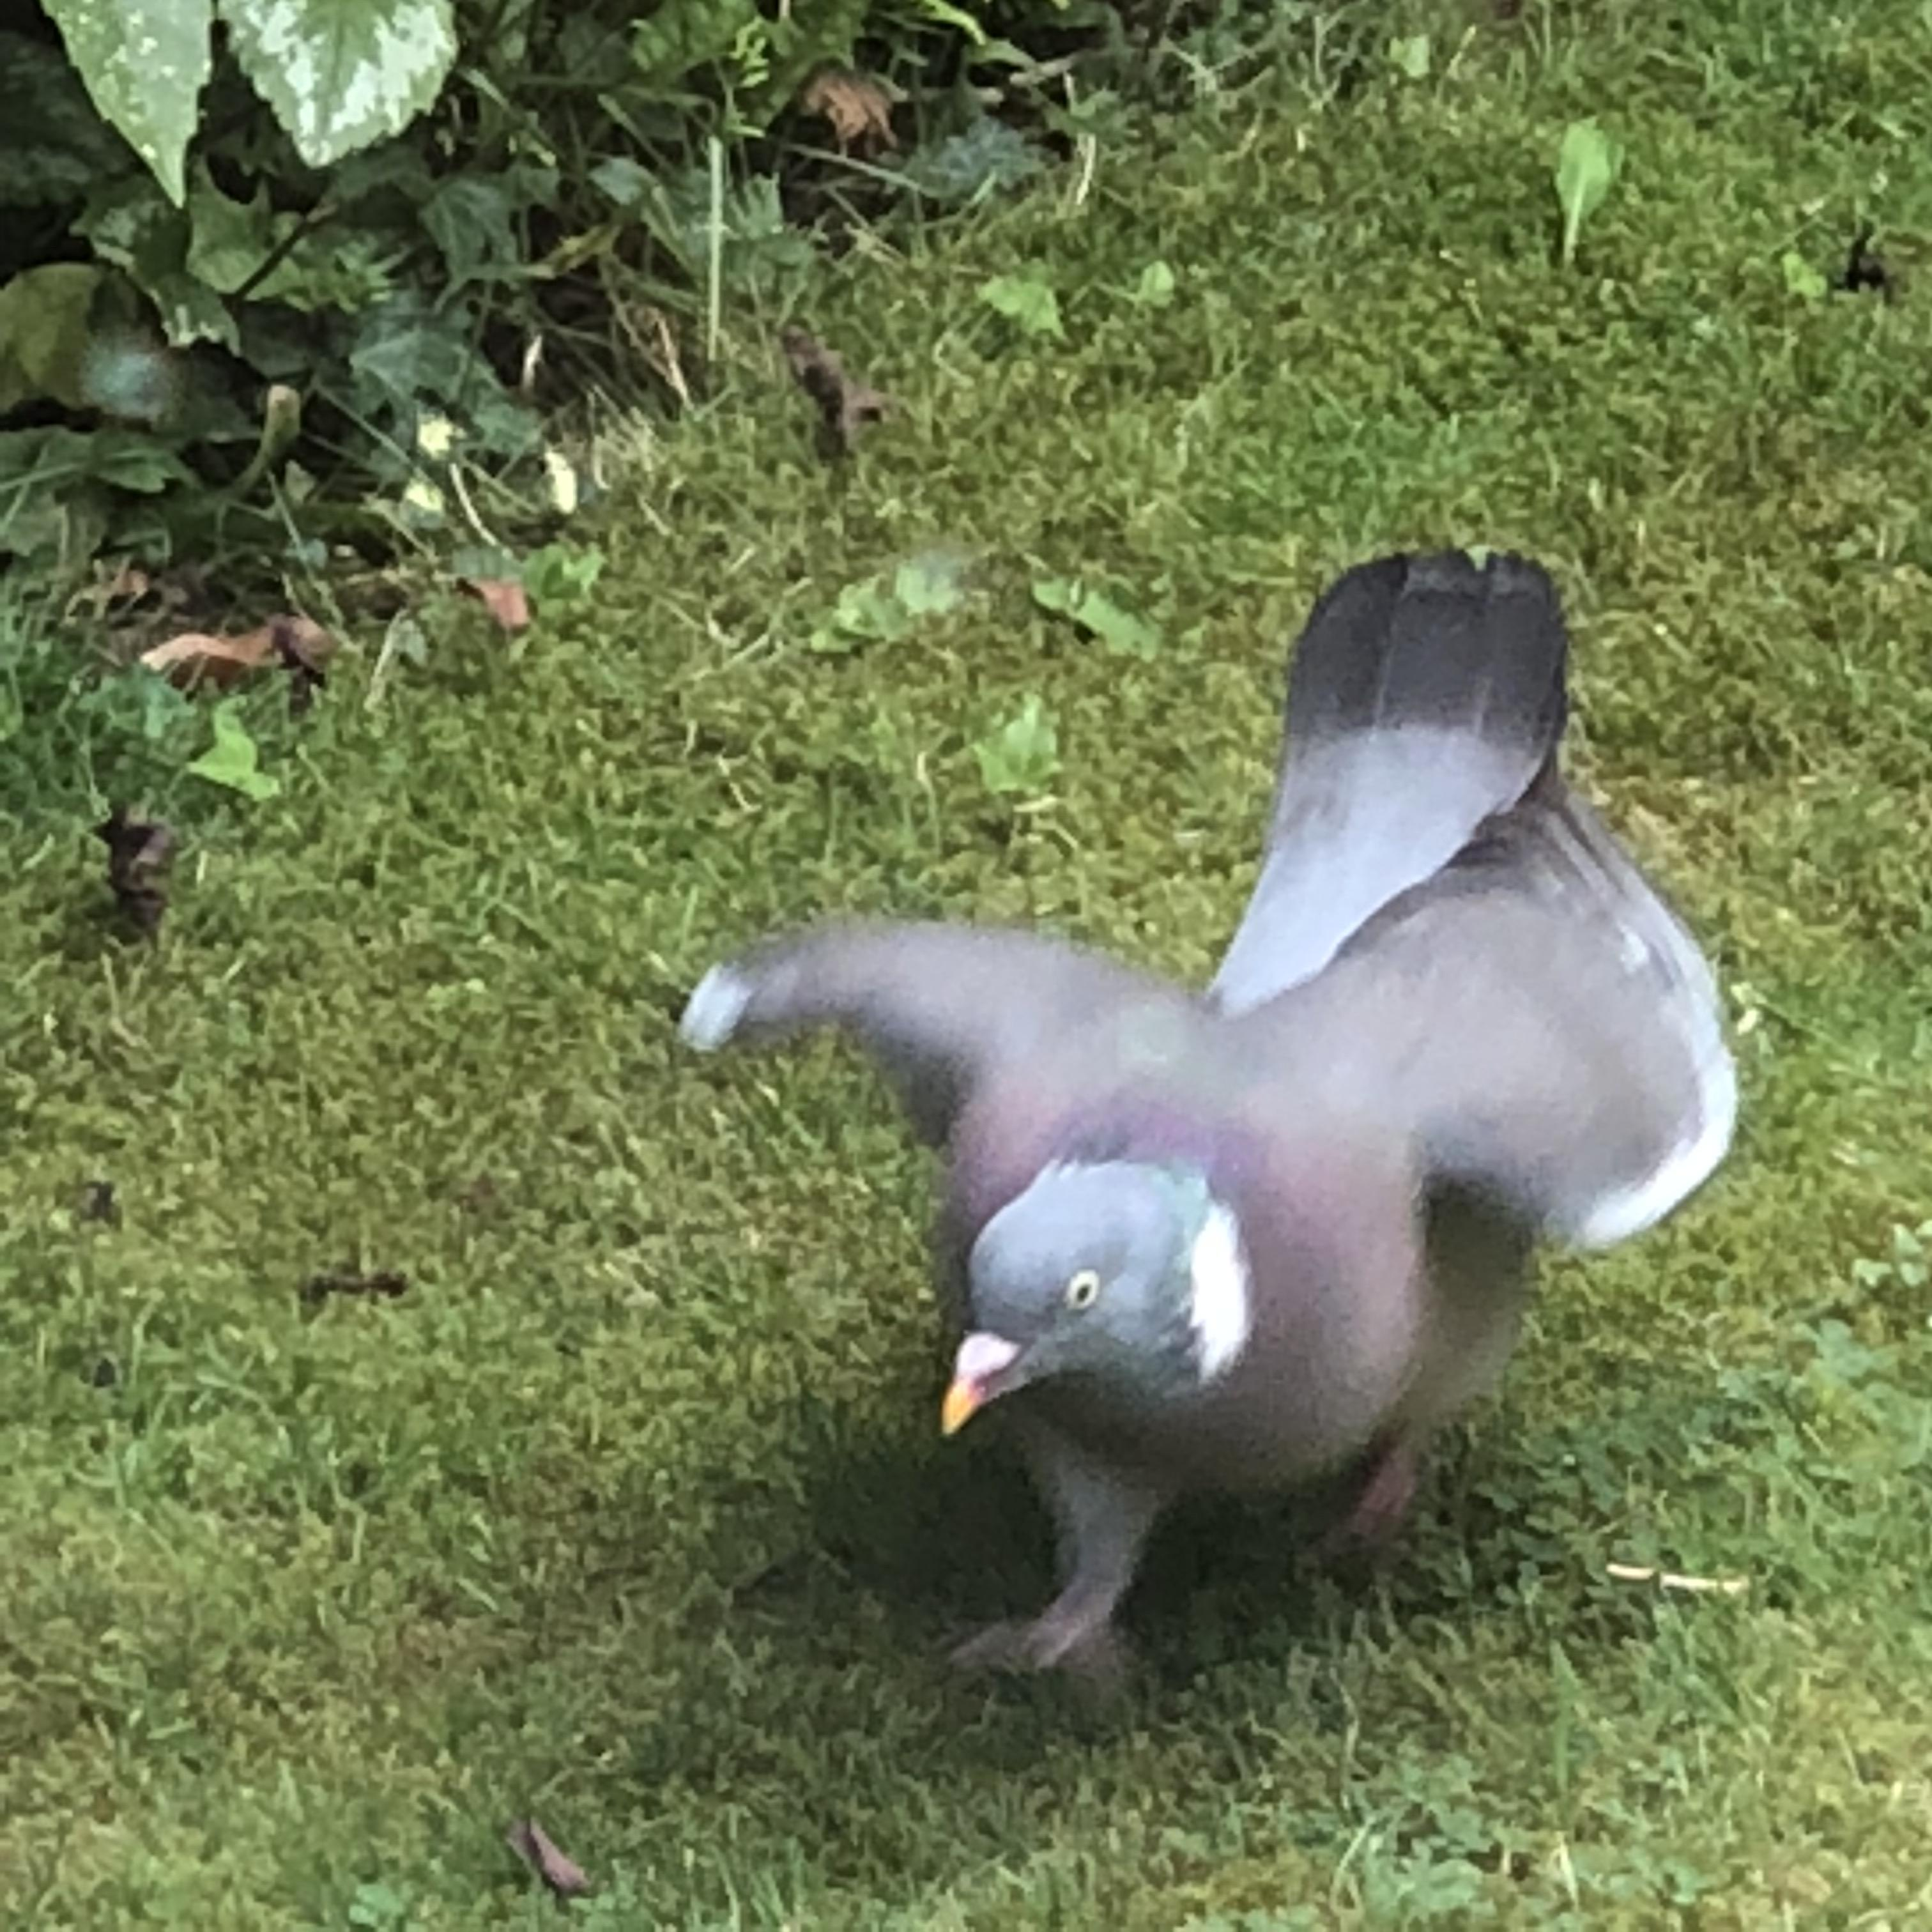
\includegraphics[width=0.9\textwidth]{graphics/bird.jpg}
        \caption[Tierforschung Beispiel Katze]{Eine Katze auf der Jagd}
        \label{fig:appendix_bird}
    \end{figure}